\documentclass[14pt, a4paper, simple]{eskdtext}

\usepackage[utf8]{inputenc}
\usepackage[russian]{babel}
\usepackage[T2A]{fontenc}
\usepackage{fancyhdr}

\usepackage{../_styles/title_variables}
\usepackage{../_styles/eskd_variables}
\usepackage{../_styles/tableOfContent}
\usepackage{../_styles/sourceCode}
\usepackage{graphicx}

\sloppy
\begin{document}
    \ESKDstyle{empty}
    \begin{flushright}
    \textbf{Приложение Б}
\end{flushright}
\begin{center}
    МИНИСТЕРСТВО ОБРАЗОВАНИЯ РЕСПУБЛИКИ БЕЛАРУСЬ

    УЧРЕЖДЕНИЕ ОБРАЗОВАНИЯ

    КАФЕДРА ИНТЕЛЛЕКТУАЛЬНЫХ ИНФОРМАЦИОННЫХ ТЕХНОЛОГИЙ
\end{center}

\vfill

\begin{center}
    \TitlePageTopic
\end{center}

\vfill

\begin{center}
    Графические материалы
\end{center}

\vfill

\begin{center}
    \graphicalAttachmentSignature
\end{center}

\vfill


\begin{center}
    Листов~\pageref{LastPage}
\end{center}

\vfill

\begin{flushright}
    \begin{minipage}[t]{7cm}
        Руководитель

        \vspace{4mm}

        Выполнил

        \vspace{4mm}

        Консультант

        по ЕСПД
    \end{minipage}
    \begin{minipage}[t]{7cm}
        \titlePageTeacherSurname~\titlePageTeacherName

        \vspace{4mm}

        \titlePageStudentSurname~\titlePageStudentName

        \vspace{4mm}

        \titlePageTeacherSurname~\titlePageTeacherName
    \end{minipage}
\end{flushright}

\vfill

\begin{center}
    \titlePageCity~\ESKDtheYear
\end{center}



    \ESKDstyle{formII}
    \begin{figure}[ht]
        \begin{center}
            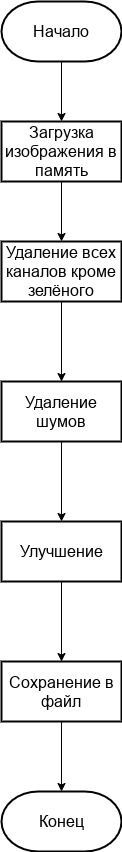
\includegraphics[width=0.17\textwidth]{../resources/shemas/shema1}
        \end{center}
        \caption{Схема алгоритма программы последовательной обработки.}
    \end{figure}
    \begin{figure}[ht]
        \begin{center}
            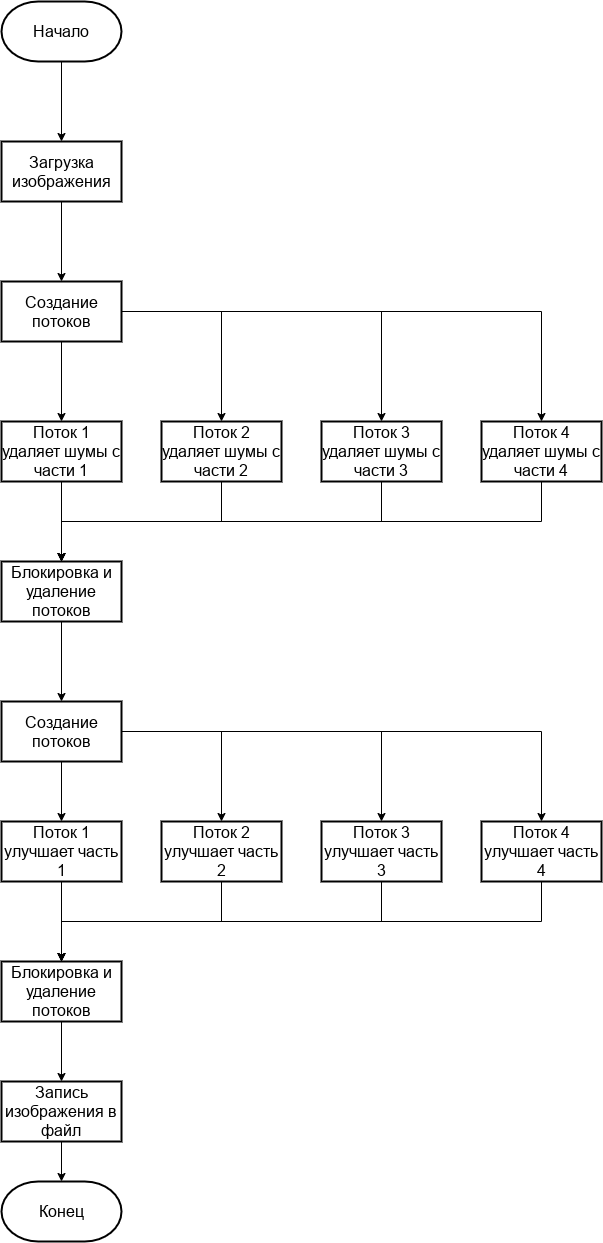
\includegraphics[width=0.6\textwidth]{../resources/shemas/shema2}
        \end{center}
        \caption{Схема алгоритма программы параллельной обработки.}
    \end{figure}
    \begin{figure}[ht]
        \begin{center}
            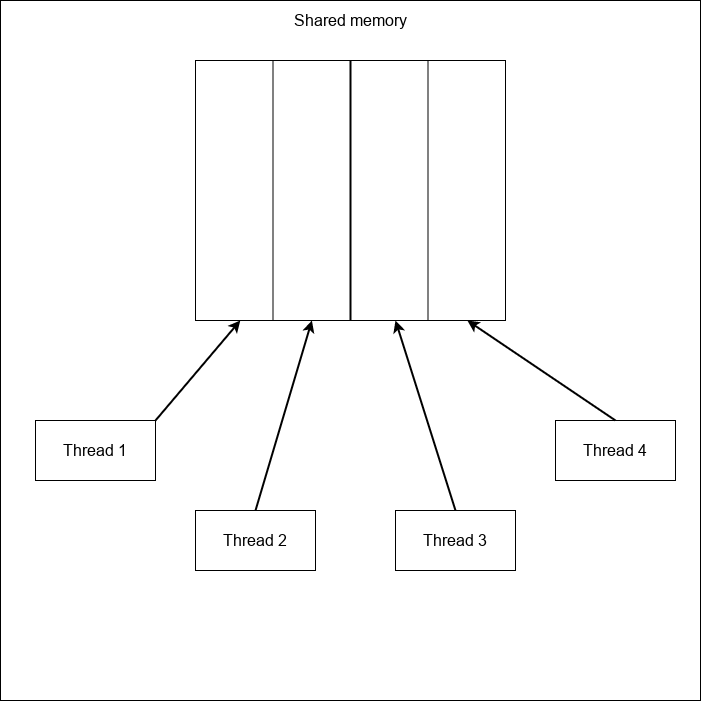
\includegraphics[width=0.9\textwidth]{../resources/shemas/shema3}
        \end{center}
        \caption{Схема ресурсов системы параллельной обработки.}
    \end{figure}
\end{document}